\documentclass[11pt, a4paper, twoside]{article}

\usepackage{fontspec}
\usepackage{blindtext}
\usepackage{geometry}
\usepackage{setspace}
\usepackage{titlesec}
\usepackage{indentfirst}
\usepackage{graphicx}
\usepackage[italian]{babel}
\usepackage{catchfile} % used in \getenv command
\usepackage{multicol}
\usepackage{amsmath}
\usepackage{subcaption}
\usepackage[hang, flushmargin, multiple, bottom]{footmisc}
\usepackage{float}
\usepackage{array}
\usepackage{booktabs}
\usepackage{url}

\raggedbottom

\titlespacing*{\section}{0px}{3mm}{1mm}
\titlespacing*{\subsection}{0px}{3mm}{1mm}
\geometry{
  left=2cm,
  right=2cm,
  top=2cm,
  bottom=2cm
}
\setlength{\parindent}{10mm}
\graphicspath{ {./assets}, {../../assets} }

% Allow use of command \getenv{VARNAME}.
% Taken from: https://tex.stackexchange.com/questions/62010/can-i-access-system-environment-variables-from-latex-for-instance-home
\newcommand{\getenv}[2][]{
  \CatchFileEdef{\temp}{"|kpsewhich --var-value #2"}{\endlinechar=-1}%
  \if\relax\detokenize{#1}\relax\temp\else\let#1\temp\fi}

% Roman numerals
\newcommand{\rom}[1]{\uppercase\expandafter{\romannumeral #1\relax}}

\begin{document}

%\begin{center}
{
	{\Large
		{\textsc{Alma Mater Studiorum $\cdot$ Università di Bologna}}
	}
}
\rule[0.1cm]{18cm}{0.1mm}
\rule[0.5cm]{18cm}{0.6mm}
{\small
	{\bf SCUOLA DI SCIENZE\\
		Corso di Laurea in Fisica
	}
}
{\let\newpage\relax\maketitle}
\end{center}


\begin{center}
  \huge Misura della caratteristica I-V di due diodi a semiconduttore \\
  \large Giuseppe Sguera \getenv{MAT1}. Matteo Bonacini \getenv{MAT2}.\\ % see readme on how to use this
  \normalsize Turno 1, tavolo (numero non indicato).\\
  \today
\end{center}

\begin{abstract}\label{sec:abstract}
  In questa prova abbiamo misurato l'andamento I-V di due diodi a semiconduttore diversi (Silicio e Germanio), per poi svolgere un \emph{fit}
  sui dati raccolti e ricavare i parametri $I_0$ e $\eta V_T$. La prova è servita anche come addestramento per usare
  un oscilloscopio analogico. I risultati dei \emph{fit} sono ?? %todo compatibili/non.
\end{abstract}

\section{Introduzione}\label{sec:scopo}
  La caratteristica I-V di un diodo al silicio contiene tutte le informazioni necessarie per descriverne il comportamento.
  Per correnti piccole, l'andamento previsto dalla teoria è riassunto nnell'Equazione di Shockley
  \begin{equation}
    I(V) = I_0 \left(
      e^{
        \frac {V_d} {\eta V_t}
      } - 1
    \right)
    \label{eq:shockley}
  \end{equation}
  dove $V_d$ è la tensione applicata ai capi del diodo, $\eta$ è il \emph{fattore di idealità}, $V_T$ è un parametro dipendente dalla
  temperatura e $I_0$ è il valore numerico della corrente inversa. Per ulteriori informazioni, si rimanda a \cite{halkias2001integrated}.
  % todo che cabbo è la corrente inversa porcoddio
  Aumentando la corrente oltre una certa soglia, l'andamento diventa sub-esponenziale e non rispetta più l'equazione \eqref{eq:shockley}.

  Lo scopo principale di questa prova è di misurare l'andamento I-V di due diodi a semiconduttore diversi (vedi sezione \ref{subsec:materiali}), per poi svolgere un
  \emph{fit} del loro andamento nel limite della validità dell'equazione \eqref{eq:shockley}. Dal fit verranno estratti i parametri $I_0$ e $\eta V_T$. 
  In secondo luogo, questa prova serve anche come addestramento per imparare ad usare un oscilloscopio analogico, in funzione delle successive
  prove di laboratorio.


\section{Apparato sperimentale}\label{sec:apparato-sperimentale}
  \subsection{Schema del circuito}\label{subsec:schema-circuito}
    \begin{figure}[H]
      \centering
      \begin{subfigure}[t]{.47\textwidth}
        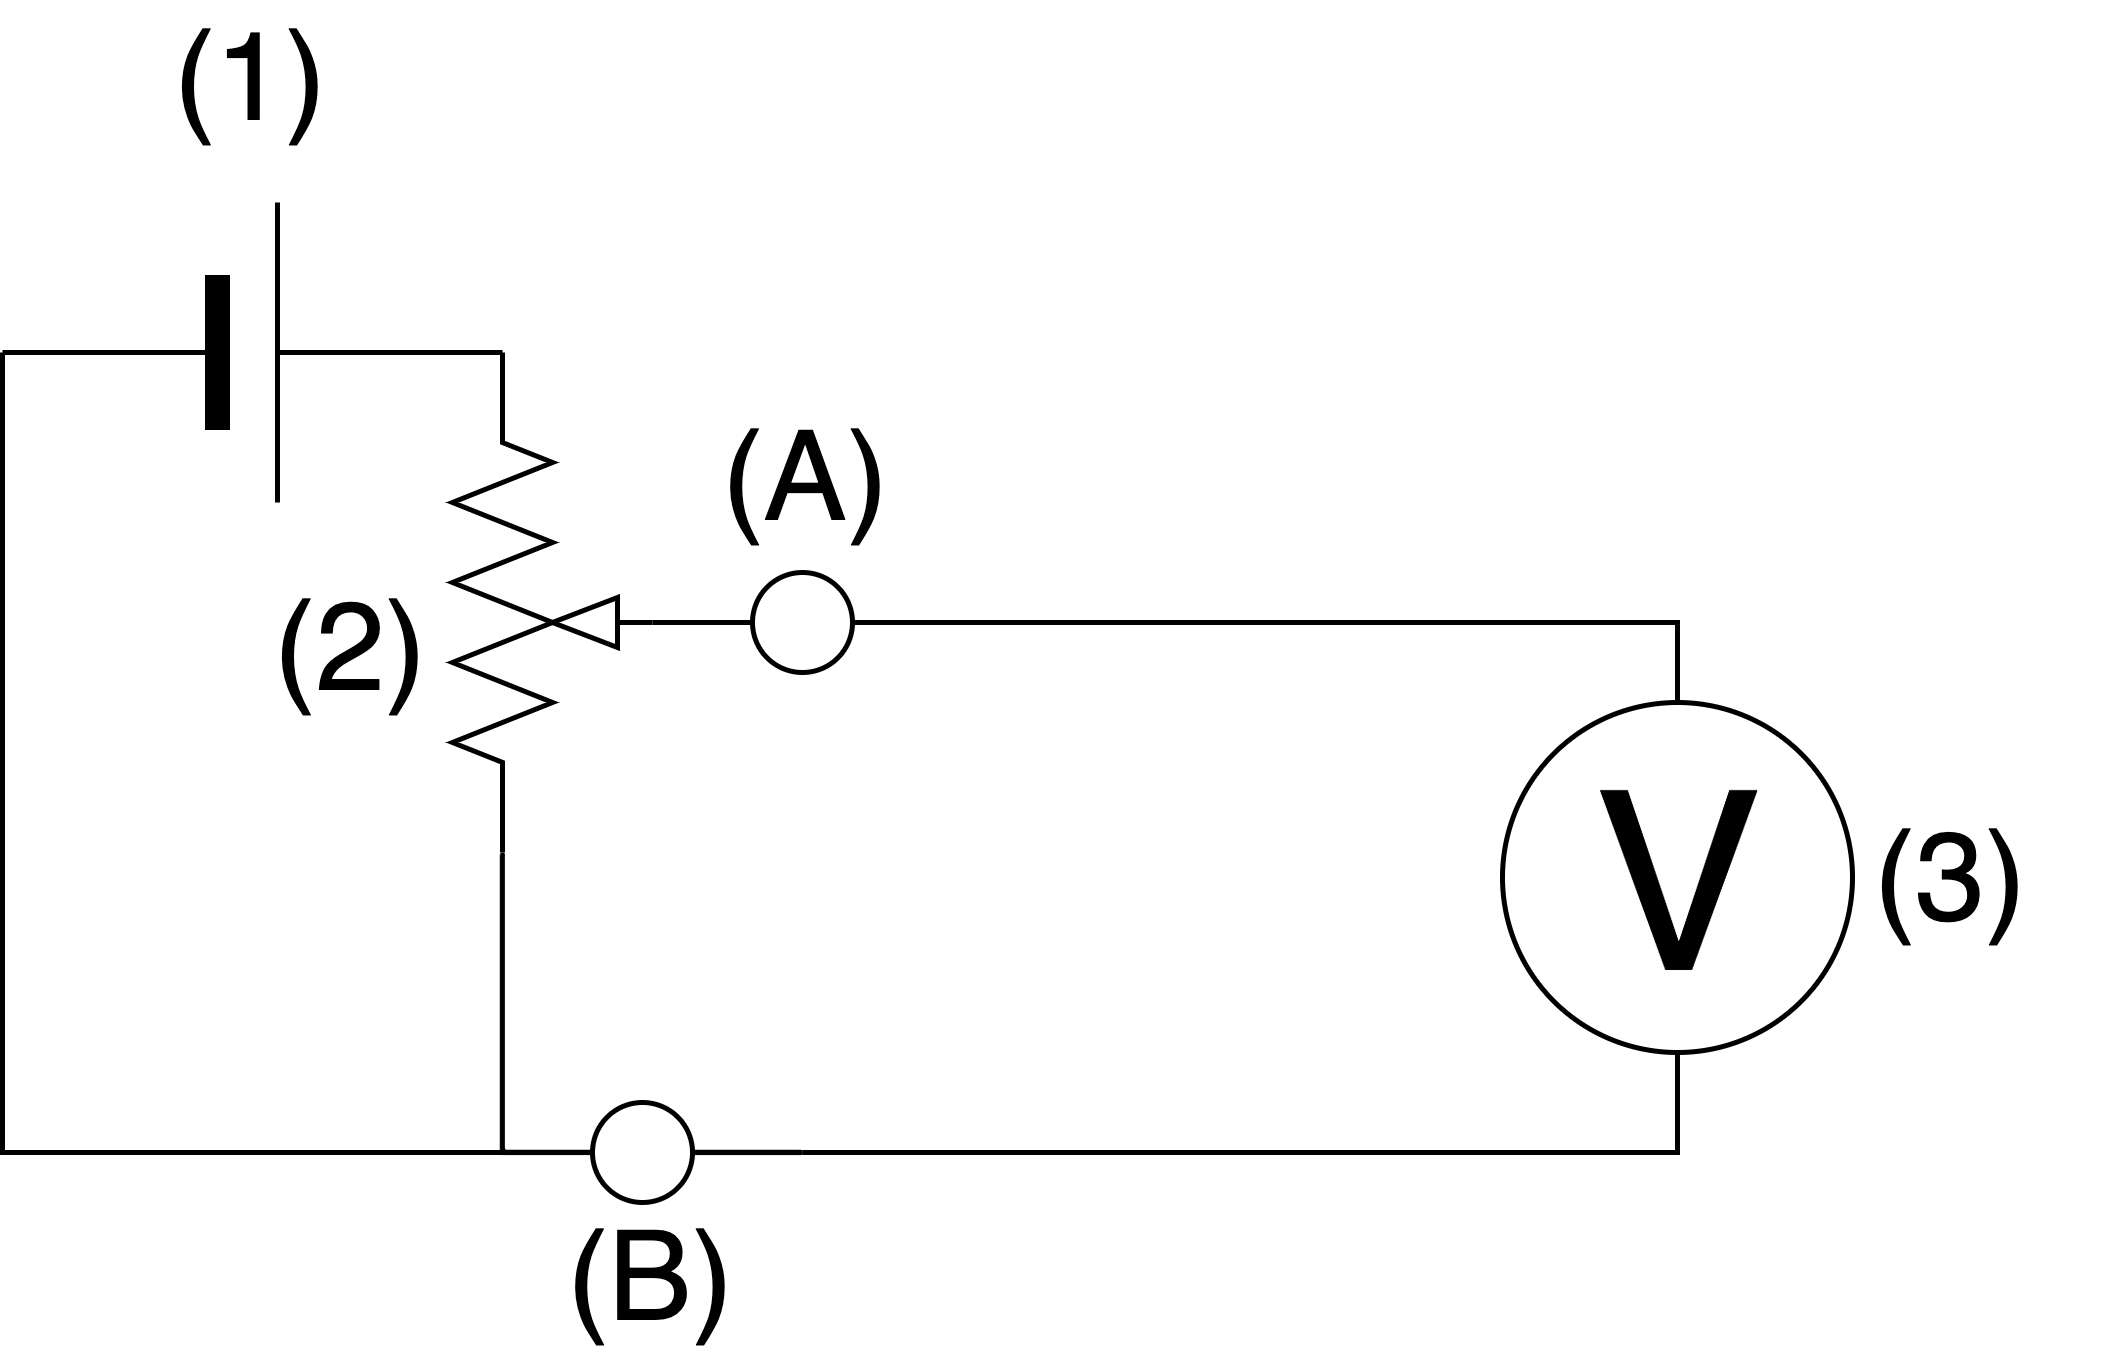
\includegraphics[width=8.75cm]{./assets/1/circuito-calibrazione.png}
        \caption{
          \emph{
            Schema del circuito usato per la calibrazione. Il generatore (1) è collegato ad un potenziometro (2).
            Il multimetro (3) misura il potenziale tra terra e il pin intermedio del potenziometro.
            L'oscilloscopio (non riportato) è collegato a terra e al punto (A).
          }
        }
        \label{fig:circuito-calibrazione}
      \end{subfigure}
      %
      \hspace{5mm}
      %
      \begin{subfigure}[t]{.47\textwidth}
        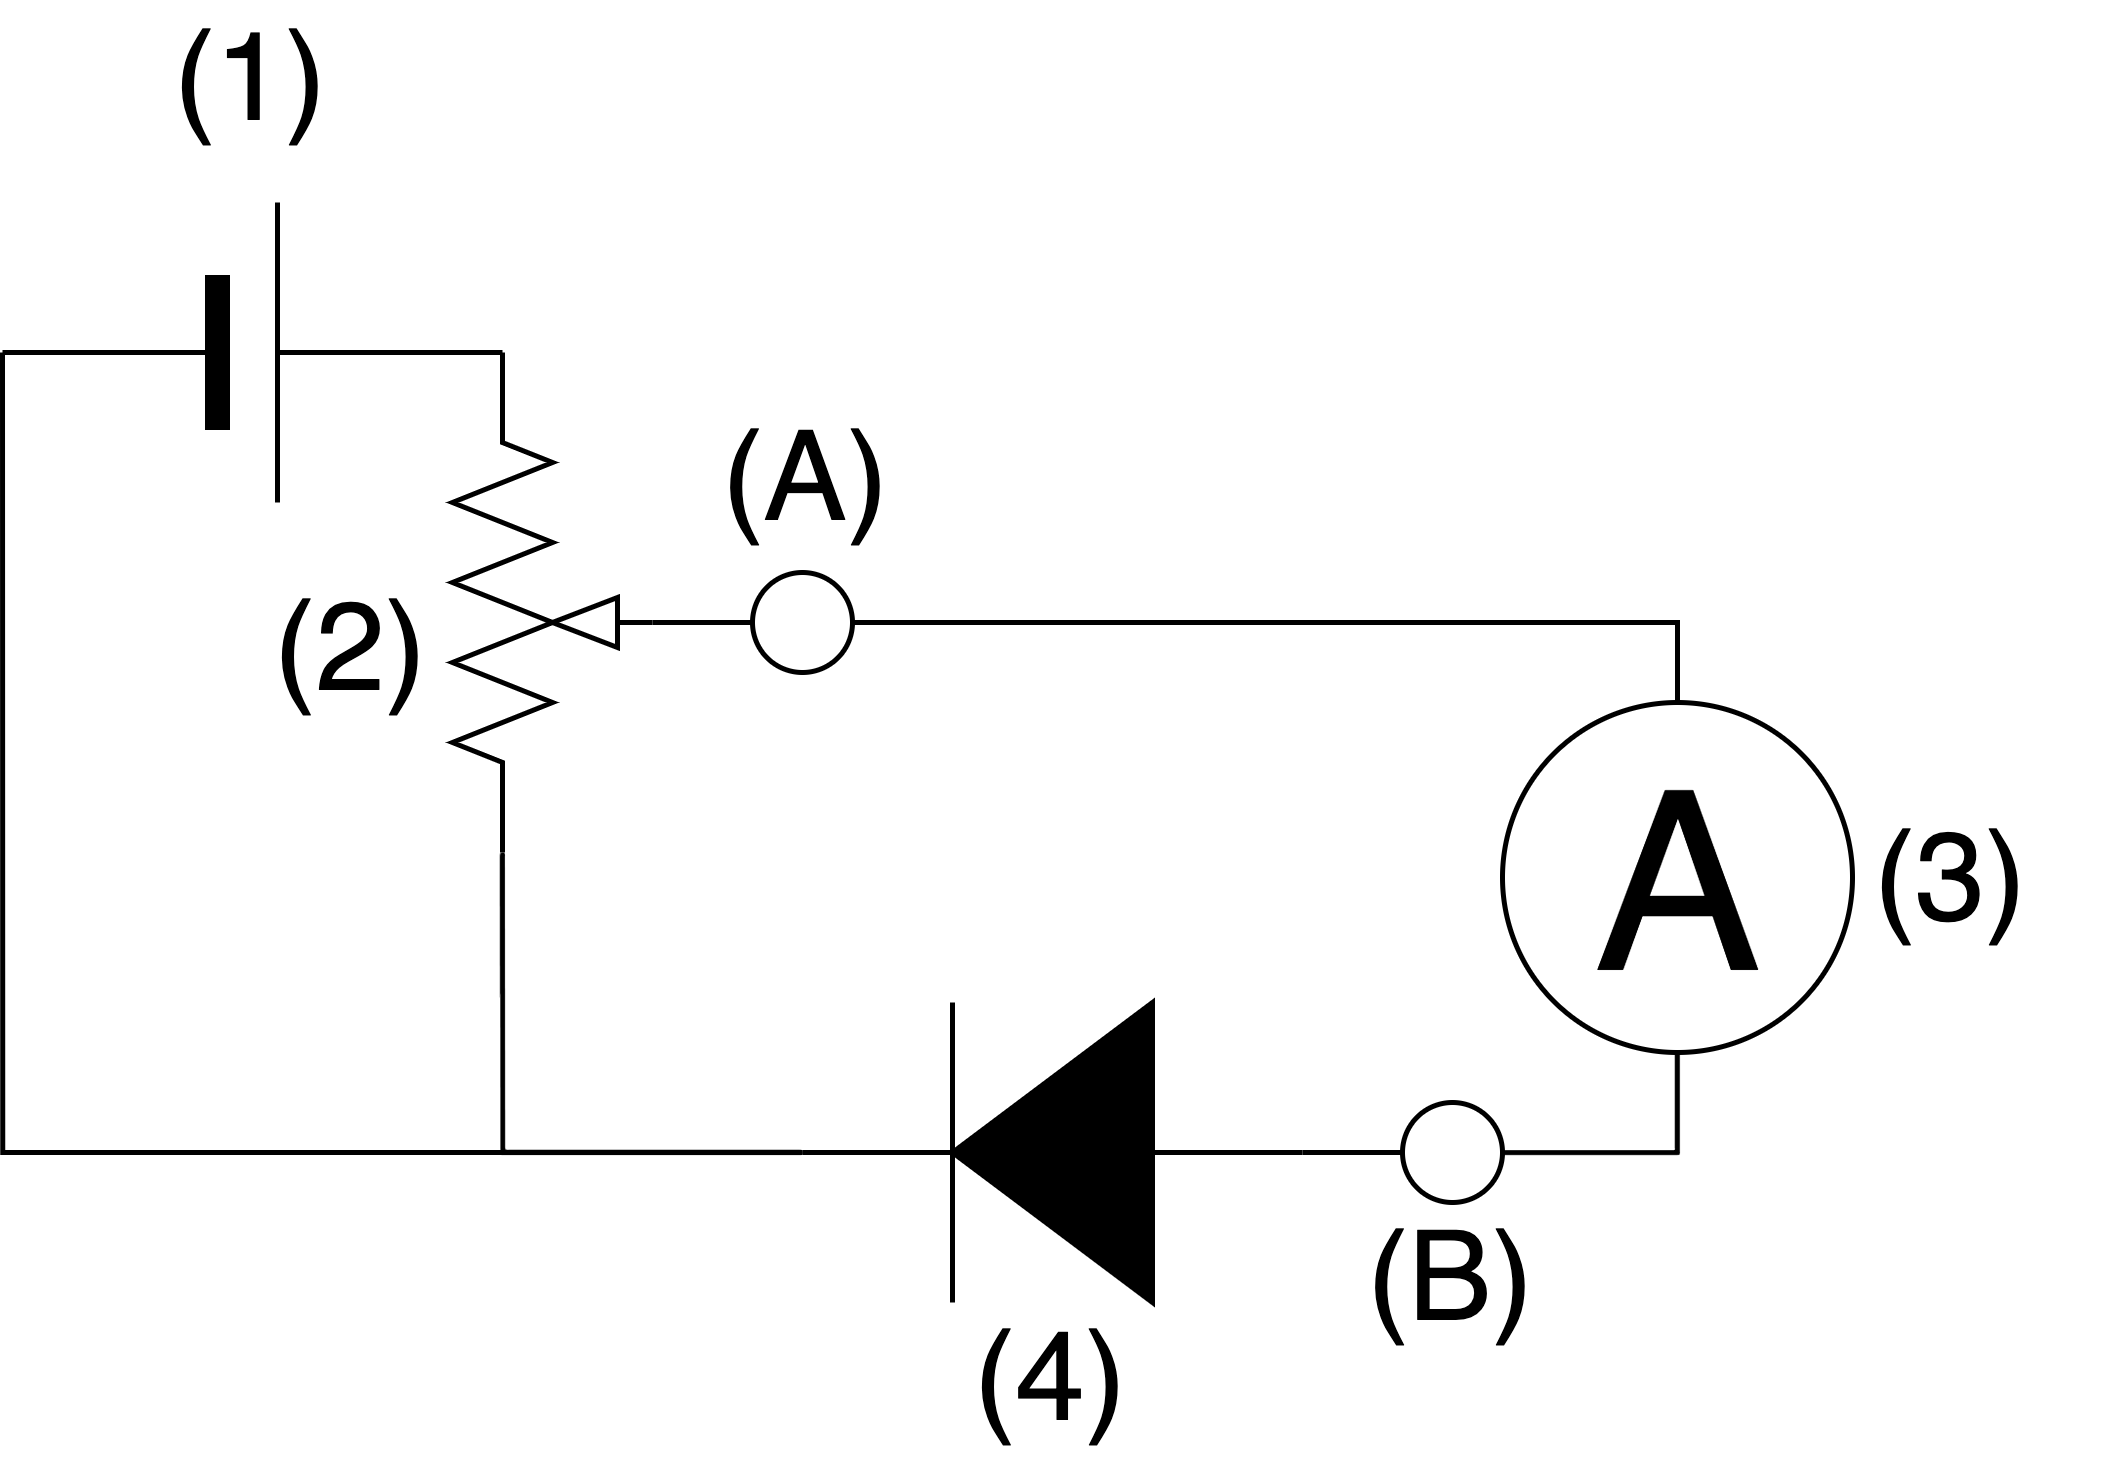
\includegraphics[width=8.75cm]{./assets/1/circuito.png}
        \caption{
          \emph{
            Schema del circuito usato per l'esperimento. Il generatore (1) è collegato ad un potenziometro (2).
            Il multimetro (3) misura la corrente che scorre nel diodo (4). L'oscilloscopio (non riportato) è
            collegato a terra e al punto (B).
          }
        }
        \label{fig:circuito-prova}
      \end{subfigure}
      \caption{\emph{Schemi circuitali.}}
      \label{fig:circuiti}
    \end{figure}

    % fixme svolgimento?
    Il circuito che abbiamo realizzato è schematizzato in figura \ref{fig:circuiti}, in due configurazioni diverse. In figura \ref{fig:circuito-calibrazione}
    è riportata la configurazione usata per controllare la calibrazione degli strimenti; in figura \ref{fig:circuito-prova}
    è riportata quella usata durante l'esperimento. In questa sezione tratteremo solamente la configurazione usata durante l'esperimento;
    la calibrazione degli strumenti verrà trattata in %todo add ref (e capire se aggiungere la sezione svolgimento)
    . Il circuito è strutturato come segue:
    \begin{enumerate}
      \item%
        Un generatore di tensione costante di $5V$ è collegato ai \emph{pin} fissi di un potenziometro.
      \item%
        Il \emph{pin} variabile del potenziometro è collegato in serie a un multimetro e a un diodo.
      \item%
        Un osciolloscopio è collegato a terra e al punto $(B)$ del circuito. 
    \end{enumerate}

  \subsection{Materiale e strumenti usati}\label{subsec:materiali}
    Segue una lista del materiale e degli strumenti usati durante la prova:
      \begin{itemize}
        \item%
          Oscilloscopio analogico, modello: %todo add modello
        \item%
          Multimetro digitale, modello: %todo add modello
        \item%
          Generatore di tensione, modello: %todo
        \item%
          Sonda per oscilloscopio.
        \item%
          Connettori vari (connettori \emph{a banana}, fili per la scheda millefori).
        \item%
          Diodo al Silicio, modello: %todo
        \item% 
          Diodo al Germanio, modello: %todo
      \end{itemize}
    Le incertezze degli strumenti utilizzati, sono riportati in appendice \ref{sec:incertezze-strumentali}.

  \subsection{Svolgimento}\label{subsec:svolgimento}
  %todo
  Non so se questa sezione lei la voglia o no...

\section{Risultati}\label{sec:risultati}
  I valori numerici dei dati raccolti sono riportati in appendice \ref{sec:valori-misure}.
  I risultati dei \emph{fit} sono riportati in tabella \ref{tab:risultati-fit}.
  In figura \ref{fig:caratteristiche-iv} sono riportati i grafici delle caratteristiche I-V dei due diodi.
  \begin{table}[H]
    \centering
    \begin{tabular}[t]{ccc}
      \toprule
      Diodo& Parametro &Valore ottenuto\\
      \midrule
      Si & $I_0$ &  $500A$ \\
      Si & $\eta V_T$ &  $500A$ \\
      Ge & $I_0$ &  $500A$ \\
      Ge & $\eta V_T$ &  $500A$ \\
      \bottomrule
      \end{tabular}
    \caption{
      Risultati dei \emph{fit} dei dati raccolti.
    }
    \label{tab:risultati-fit}
  \end{table}
  %todo potenzialmente aggiungi calcolo di V_T??
  %todo aggiungi considerazioni sull'andamento.
  \begin{figure}[H]
    \centering
    \begin{subfigure}[t]{.47\textwidth}
      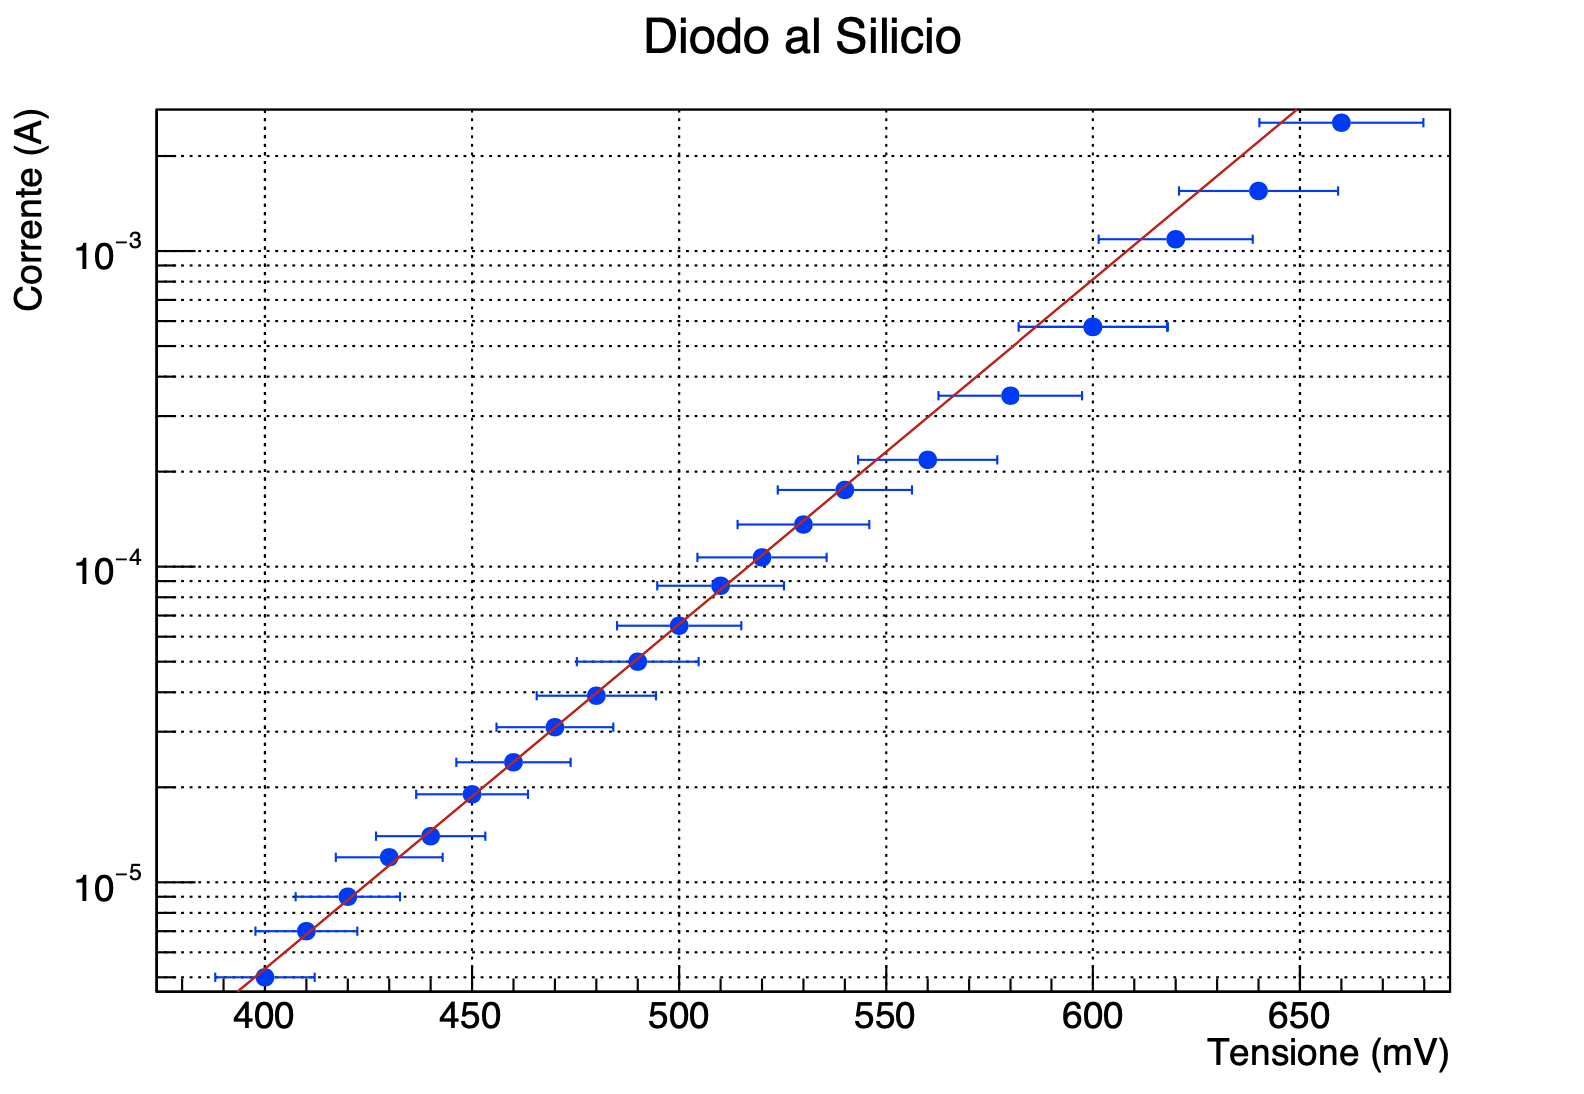
\includegraphics[width=8.25cm]{./assets/1/silicio.png}
      \caption{
        \emph{
          Caratteristica I-V del diodo al Silicio. Sono riportati i dati raccolti, assieme al fit lineare svolto sui primi punti.
        }
      }
      \label{fig:caratteristica-silicio}
    \end{subfigure}
    %
    \hspace{5mm}
    %
    \begin{subfigure}[t]{.47\textwidth}
      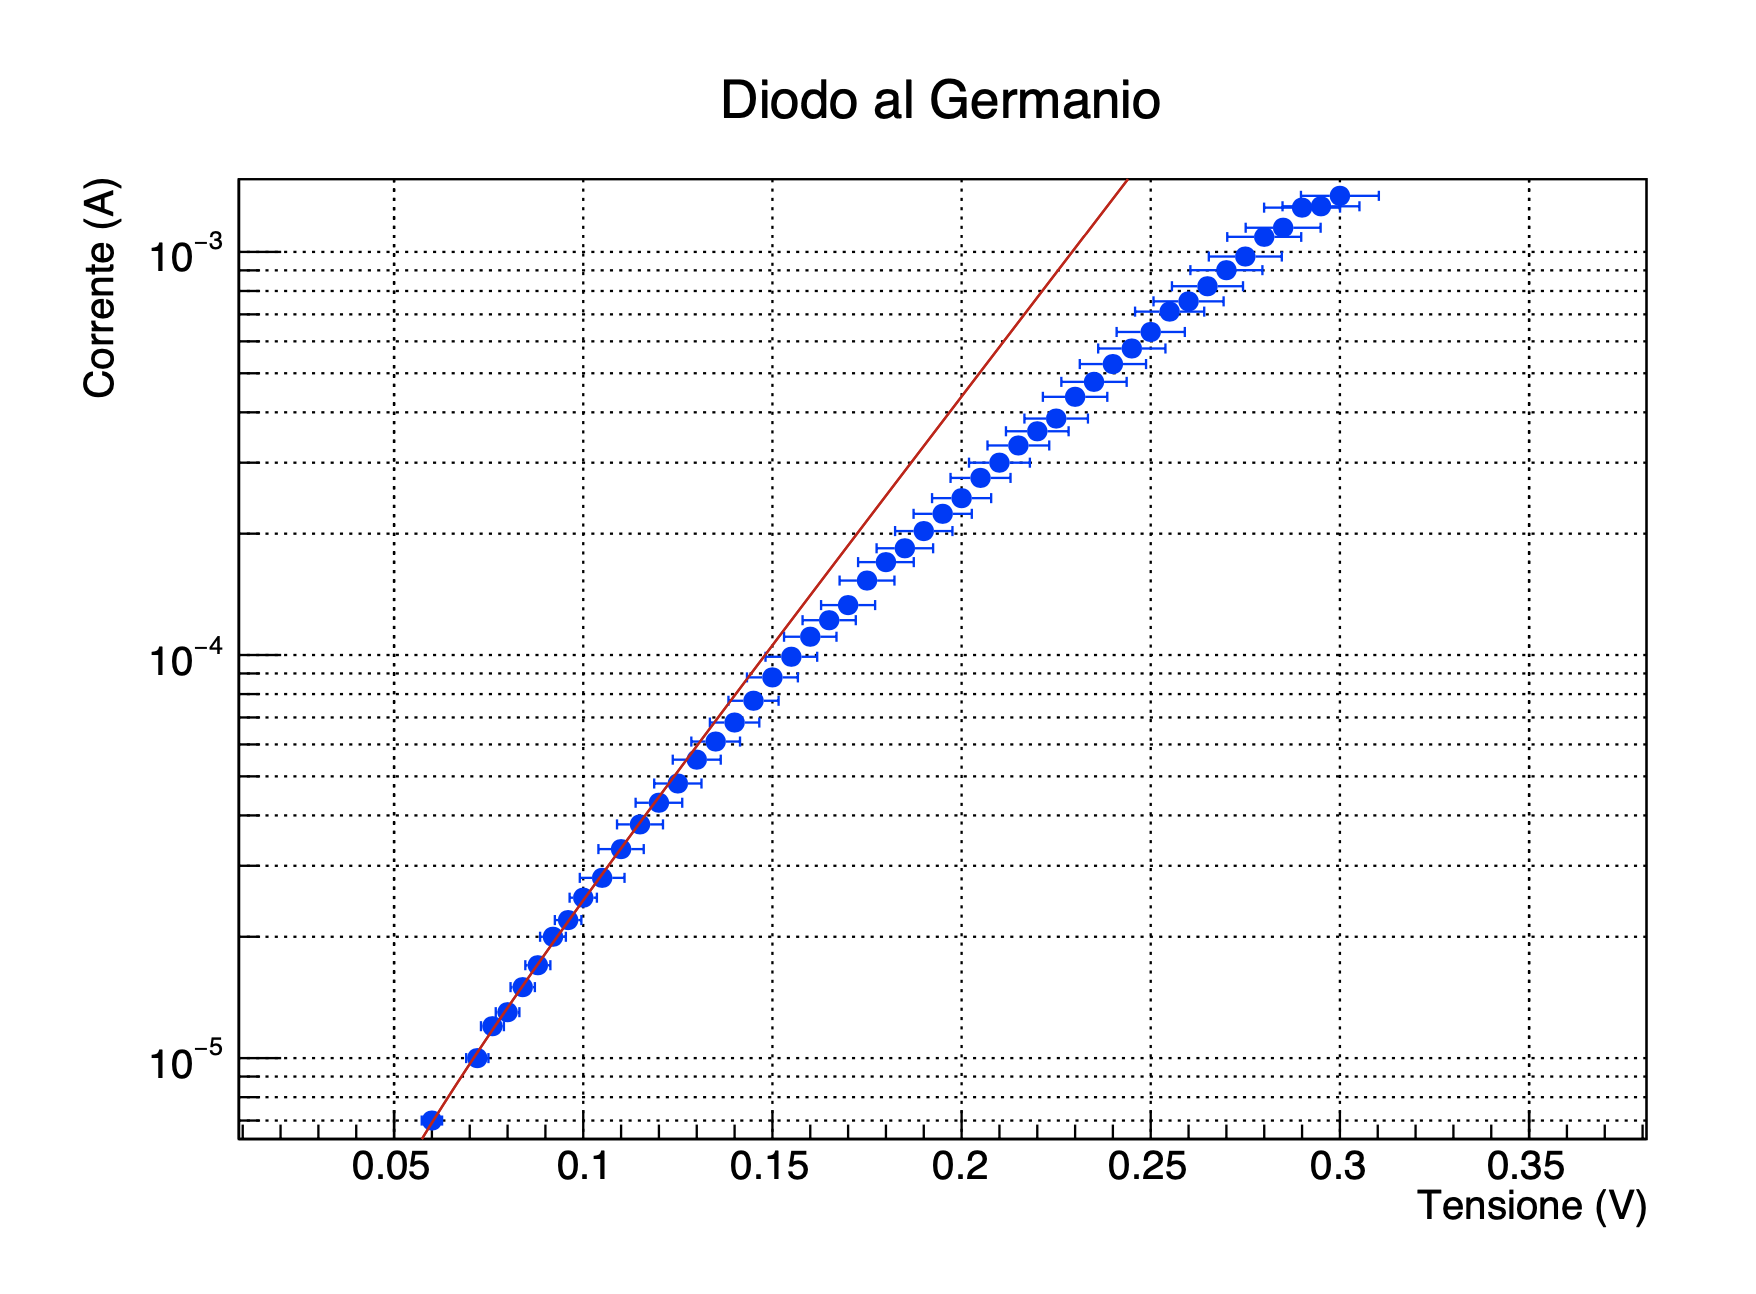
\includegraphics[width=8.25cm]{./assets/1/germanio.png}
      \caption{
        \emph{
           Caratteristica I-V del diodo al Germanio. Sono riportati i dati raccolti, assieme al fit lineare svolto sui primi punti.
        }
      }
      \label{fig:caratteristica-germanio}
    \end{subfigure}
    \caption{\emph{Dati raccolti.}
    \label{fig:caratteristiche-iv}}
  \end{figure}

\section{Conclusioni}\label{sec:conclusioni}
  C'è da capire se vuole questa roba

\newpage
\appendix
\textbf{\huge{Appendice}}
\section{Incertezze strumentali}\label{sec:incertezze-strumentali}
  culo2

\section{Valori numerici delle misure}\label{sec:valori-misure}
  %todo 
  culo

\bibliographystyle{unsrt} % We choose the "plain" reference style
\bibliography{./docs/reports/electronicsLabRefs.bib}

\end{document}
